\documentclass[11pt]{beamer}
\usepackage[utf8]{inputenc}
\usepackage[T1]{fontenc}
\usepackage{lmodern}
\usepackage[english]{babel}
\usepackage{amsmath}
\usepackage{amsfonts}
\usepackage{amssymb}
\usepackage{graphicx}
\usetheme{default}
\begin{document}
	\author{Nayani Jani\\
		Christopher Odoom\\
		Denis Folitse\\
		Animesh Sengupta\\ }
	\title{\bf{A Quasi-Poisson Approach\\ Goals in Football, What contributes to them? }}
	%\subtitle{}

	\institute{\textbf{   University of Massachusetts, Amherst }}
	%\date{}
	%\subject{}
	%\setbeamercovered{transparent}
	%\setbeamertemplate{navigation symbols}{}
	\begin{frame}[plain]
		\maketitle
	\end{frame}
	
\begin{frame}	
		\frametitle{Background of study}
		Football has become a part of the world and is one of the biggest source of entertainment in the world. It has created job and opportunities to people all over the world. It's important in this modern time cannot be overlooked.There are five major football leagues in the world; English premier league, German BundesLiga, Spanish Laliga, Italian Seria A and France League one. Football supporters of English primier league all over the world always claim that, their league is the difficult one among all the five major leagues, is this claim true?. Football fans all over the world have insufficient answer to this question. This study tries to provide answer to this question.
		
	\end{frame}

	
	\begin{frame}
		\frametitle{Problem statement}
	Argument: If a league has a lot of goals scored in a season it is deemed not competitive because of the quality of opponents (vice versa as well).
	Goal: Does the factor league determine the amount of goals combined with other variables? If not, what predictors are associated with the response Goals?	
	\end{frame}

	\begin{frame}
		\frametitle{Objectives}
		This study is directed by the specific objectives stated below;\\
		\begin{enumerate}
			
			
			\item Determine if there is a significant difference in goals across the 5 major leagues.
			
			\item Determine if there are other predictors that are associated with the goals other than the different leagues.
			
		\end{enumerate}
	\end{frame}

	\begin{frame}
		\frametitle{Methodology}
		This study used  a data which was collected from \url{ https://fbref.com}, 
		We used the
		2021-2022 season statistics for EPL, La Liga, Bundesliga, Ligue 1 and Serie A in the analysis. The data comprise of 98 observations and 18 variables.
		Models we considered includes
		Poisson regression,
		 Quasi - Poisson Regression.
		 
		Diagnostic Tests: Test for Overdispersion, Residual Vs. Fitted Plot, Normal QQ-Plot
	\end{frame}

\begin{frame}
	\frametitle{Poisson Regression}
	This is type a regression used when the response variable is a COUNT variable. It models the logarithm of the expected value of occurrence of an event as a linear function of some predictor variables.\\
	The mathematical equation for the model is given below:
	\[log(E(no.Goals|X))= \beta_0+\beta^{'}X\]
	Alternatively, we can write it in an exponential form as:
	\[E(No.Goals|X)= e^{(\beta_0+\beta^{'}X)}\]
	The method used here to estimate the paramters is the Maximum Liklihood estimator.	
	
\end{frame}

\begin{frame}
	\frametitle{Assumptions of poisson Regression}
	\begin{itemize}
		\item The number of goals must be scored in a fixed time.
		\item \[E(no.Gls|X) =Var(no.Gls|X)\]
	\end{itemize}
\end{frame}
\begin{frame}
	\frametitle{Estimation of parameter}
	The estimation method used here is the maximum likelihood estimation method.
	The procedure is briefly described below:
	Given the model:
	\[\lambda(x)= E(Y|X)= e^{\beta^{'}X}\]
	Here Y, the response follow a Poisson distribution, therefore we have
	\[P(y|x,\beta^{'})= \frac{\lambda(x)^y e^{-\lambda(x)}}{y!}\]   \[= \frac{e^{y \beta^{'}X} e^{-e^{\beta^{'}X}}}{y!}\]
	
	Now suppose we have  data set $(X,y)$ with n rows, then given an set of parameters $\beta$ the likelihood is given by
	\[L(\beta|X,Y)= \prod_{i=1}^{n} \frac{e^{y_i \beta^{'}X_i} e^{-e^{\beta^{'}X_i}}}{y_i!}\]
	The goal is to find $\beta$ which maximize this likelihood.
\end{frame}

\begin{frame}
	\frametitle{Quasi-Poisson}
	This study used this variant of Poisson regression because, the data is under-dispersed( the conditonal variance is smaller than expected).
	The type of model add a parameter called the dispersion which help solve the problem of under-dispersion. This reason for this model is to produce credible inference. 
	The dispersion parameter is given by
	\[\hat{\phi}=\frac{1}{n-K}\sum_{i=1}^{n}\frac{(y_i-\hat{y_i})^2}{\hat{y_i}}\]
	where K is the number of parameters.\\
	such that
	\[Var(Y|X)=\hat{\phi}E(Y|X) \]
	if $\hat{\phi}=1$ we have Possion regression\\
	if $\hat{\phi}>1$ we have over-dispersion\\
	if $\hat{\phi}<1$ we have under-dispersion
	
\end{frame}
\begin{frame}
	\frametitle{Pearson Residuals}
	This is a useful measure for diagnosing the appropriateness of a Poisson regression. This type of residual is a weighted residual and when ploted with the fitted points tells us if the Poisson regression is ok and there is no issue with dispersion. This measure is computed with the formula below.
	\[Pearson Residual=\frac{y_i-\hat{y_i}}{\sqrt{\hat{y_i}}}\]  
\end{frame}

\begin{frame}{Descriptive}
	\frametitle{Results}
	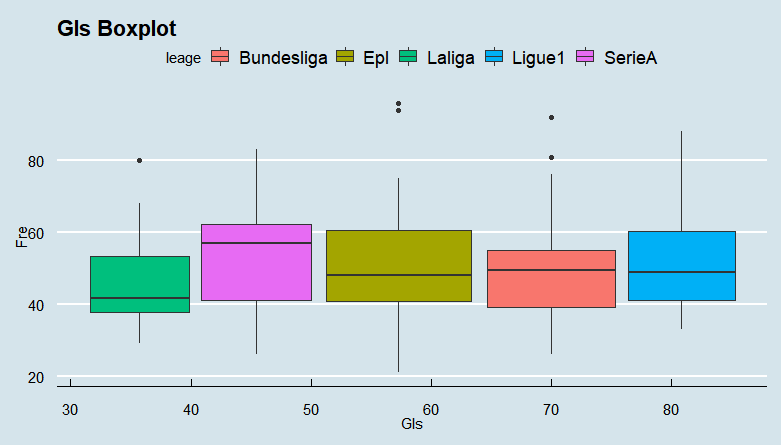
\includegraphics[scale=0.5]{Gls}
	\figurename 1: The plot show the goals distribution across the 5 Leagues
\end{frame}

\begin{frame}{Descriptive}
	\frametitle{Results}
	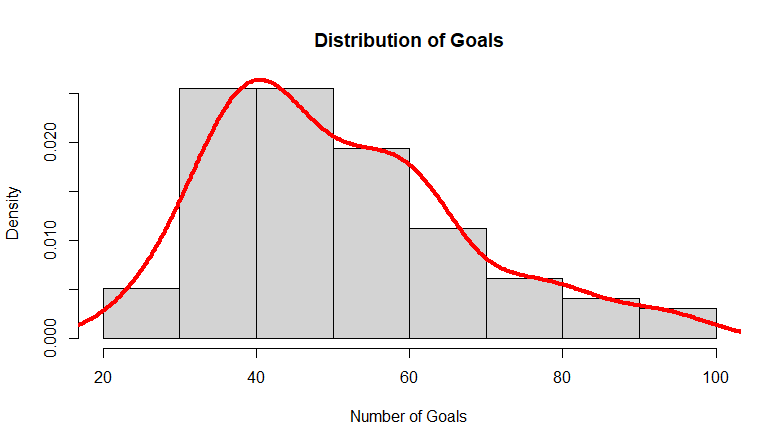
\includegraphics[scale=0.5]{gls1}
	\figurename 1: The plot show the goals distribution across the 5 Leagues
\end{frame}

\begin{frame}
	\frametitle{Results}
	\begin{tabular}{@{\extracolsep{5pt}} ccccc} 
		\\[-1.8ex]\hline 
		\hline \\[-1.8ex] 
		& Estimate & Std. Error & t value & Pr(\textgreater \textbar t\textbar ) \\ 
		\hline \\[-1.8ex] 
		(Intercept) & $2.870$ & $0.217$ & $13.222$ & $0$ \\ 
		leageBundesliga & $0.096$ & $0.045$ & $2.121$ & $0.037$ \\ 
		leageLaliga & $$-$0.003$ & $0.041$ & $$-$0.077$ & $0.939$ \\ 
		leageLigue1 & $0.032$ & $0.041$ & $0.776$ & $0.440$ \\ 
		leageSerieA & $0.009$ & $0.042$ & $0.217$ & $0.829$ \\ 
		No.Pl & $$-$0.001$ & $0.004$ & $$-$0.143$ & $0.887$ \\ 
		SoT & $0.005$ & $0.001$ & $7.661$ & $0$ \\ 
		PK & $0.044$ & $0.028$ & $1.559$ & $0.123$ \\ 
		FK & $$-$0.012$ & $0.009$ & $$-$1.373$ & $0.174$ \\ 
		Att.3rd.T & $$-$0.00001$ & $0.00002$ & $$-$0.360$ & $0.719$ \\ 
		Succ.Drib & $$-$0.001$ & $0.0003$ & $$-$1.923$ & $0.058$ \\ 
		ShortAT\_Pass & $0.00003$ & $0.00003$ & $1.049$ & $0.297$ \\ 
		NumAtt & $0.072$ & $0.013$ & $5.560$ & $0.00000$ \\ 
		PK:ShortAT\_Pass & $$-$0.00000$ & $0.00000$ & $$-$1.039$ & $0.302$ \\ 
		FK:ShortAT\_Pass & $0.00000$ & $0.00000$ & $1.165$ & $0.247$ \\ 
		\hline \\[-1.8ex] 
	\end{tabular} 
\end{table} 

\end{frame}


\begin{frame}
	\frametitle{Results}
\begin{table}[!htbp] \centering 
	\caption{Poisson Regression Output} 
	\label{} 
	\begin{tabular}{@{\extracolsep{5pt}} ccccc} 
		\\[-1.8ex]\hline 
		\hline \\[-1.8ex] 
		& Estimate & Std. Error & z value & Pr(\textgreater \textbar z\textbar ) \\ 
		\hline \\[-1.8ex] 
		(Intercept) & $2.853$ & $0.103$ & $27.592$ & $0$ \\ 
		leageBundesliga & $0.093$ & $0.053$ & $1.770$ & $0.077$ \\ 
		leageLaliga & $$-$0.007$ & $0.048$ & $$-$0.138$ & $0.890$ \\ 
		leageLigue1 & $0.036$ & $0.048$ & $0.742$ & $0.458$ \\ 
		leageSerieA & $0.004$ & $0.048$ & $0.089$ & $0.929$ \\ 
		SoT & $0.005$ & $0.001$ & $6.503$ & $0$ \\ 
		PK & $0.016$ & $0.007$ & $2.244$ & $0.025$ \\ 
		FK & $$-$0.003$ & $0.003$ & $$-$0.993$ & $0.321$ \\ 
		Att.3rd.T & $$-$0.00001$ & $0.00003$ & $$-$0.283$ & $0.777$ \\ 
		Succ.Drib & $$-$0.0005$ & $0.0003$ & $$-$1.655$ & $0.098$ \\ 
		ShortAT\_Pass & $0.00003$ & $0.00002$ & $1.885$ & $0.059$ \\ 
		NumAtt & $0.073$ & $0.015$ & $4.719$ & $0.00000$ \\ 
		\hline \\[-1.8ex] 
	\end{tabular} 
\end{table}
\end{frame}
\end{document}











